\section{Introduction}

In today's world, data has emerged as the cornerstone of decision-making, driving innovation and redefining strategies across industries. 
The evolution of data-driven technologies can be traced through several transformative phases, each contributing to the way businesses harness information for growth and efficiency.

\begin{chronology}[5]{2010}{2025}{0.9\textwidth}
    \event[2012]{2015}{Big data}
    \event[2015]{2018}{Machine Learning}
    \event[2014]{2017}{Cloud computing}
    \event[2017]{2025}{Generative AI}
\end{chronology}

\paragraph*{Big data} 
The era of Big Data began with the exponential surge in structured and unstructured data generated daily. 
This phase introduced significant challenges in terms of storage, management, and analysis, but it also opened up unprecedented opportunities for deriving business intelligence and actionable insights.

\paragraph*{Machine Learning}
Machine Learning marked a pivotal shift in data utilization, empowering computers to identify patterns and make decisions without explicit programming. 
Its applications grew rapidly, enabling predictive analytics and automation that transformed industries and streamlined operations.

\paragraph*{Cloud Computing}
Cloud computing revolutionized data infrastructure by offering scalable, cost-effective solutions accessible over the internet. 
It eliminated traditional infrastructure constraints, providing businesses with flexible computing power and facilitating seamless data processing and storage.

\paragraph*{Generative Artificial Intelligence}
Generative AI represents the cutting edge of technological advancement, where systems exhibit human-like understanding and creativity. 
These AI models are capable of producing new content, analyzing complex datasets, and solving problems across diverse domains, reshaping industries and redefining how humans interact with technology.

\begin{figure}[H]
    \centering
    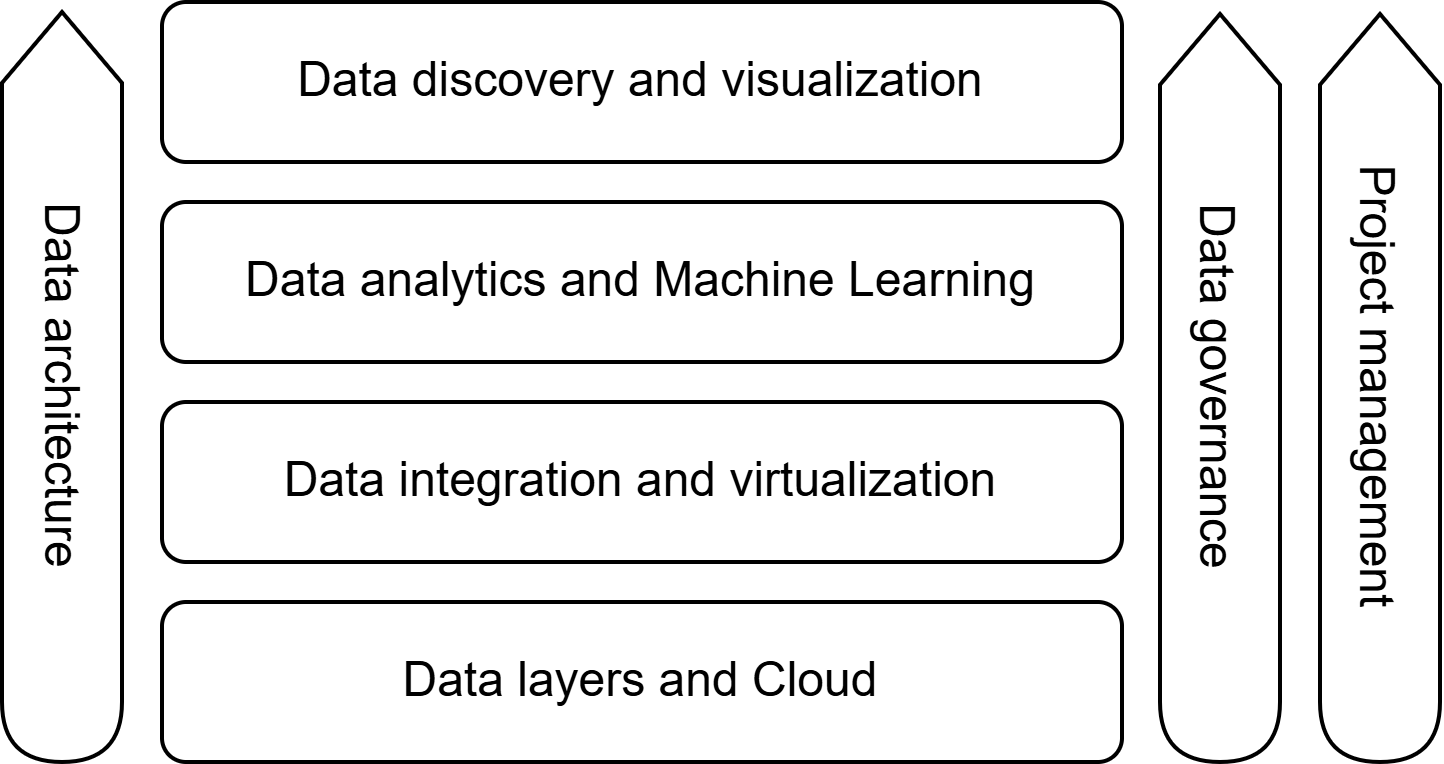
\includegraphics[width=0.5\linewidth]{images/bis10.png}
    \caption{Data framework}
\end{figure}

The growing importance of data has given rise to specialized roles critical to managing and leveraging this resource effectively:
\begin{itemize}
    \item \textit{Data and Cloud architect}: design robust data infrastructures aligned with business goals, ensuring efficient integration and optimal storage. 
        Cloud architects focus on building scalable, cloud-based systems to meet modern data demands.
    \item \textit{Data engineer}: develop and maintain systems for collecting, processing, and storing data.
        They design ETL pipelines, work with big data tools, and transform raw data into formats suitable for analysis.
    \item \textit{Data analyst}:  interpret datasets to extract meaningful insights. 
        They clean and analyze data, perform statistical evaluations, and create visualizations to guide strategic decisions.
    \item \textit{Data scientist}:  apply advanced analytics and machine learning techniques to uncover patterns and predictions from complex datasets. 
        Using programming languages like Python, they drive deeper insights and develop innovative solutions.
    \item \textit{Data privacy and security specialist}: these professionals ensure compliance with data protection laws and implement robust security measures to safeguard organizational data from cyber threats and breaches.
\end{itemize}